\documentclass[10pt]{article}

\usepackage{lipsum}
\usepackage{url}
\usepackage{float}
\usepackage{amsmath}
\usepackage{enumitem}
\usepackage{graphicx}
\usepackage{caption}
\usepackage{subcaption}
\usepackage{rotating}
\usepackage{geometry}
\usepackage{listings}
\usepackage{hyperref}
\usepackage[T1]{fontenc}
\usepackage[numbered]{matlab-prettifier}

\newcommand{\documentTitle}{Lab 1 - Basic Electrical Measurements}
\newcommand{\documentAuthor}{Aneel Damaraju, Andrew Pham}
\newcommand{\courseTitle}{ELEC 240}
\newcommand{\testDate}{September 04, 2018}
\newcommand{\reportDate}{September 11, 2018}

\geometry{margin=1in}
\lstset{
	tabsize=4,
	basicstyle={\ttfamily},
	captionpos=b,
	belowskip=1em,
	aboveskip=1em,
	numbers=left,
	escapechar=\@,
}

\title{
	\textbf{\courseTitle} \\
	\textbf{\documentTitle} \\
	\bigskip
	\textbf{\large{Test performed: \testDate}} \\
	\textbf{\large{Report submitted: \reportDate}} \\
	\bigskip
	\bigskip
}
\author{\documentAuthor}
\date{}

\begin{document}
	
	\maketitle
	
	\newpage
	
	\section{Objective}
	
	This lab focuses on the fundamental tools and skills for electrical engineering laboratory work. This includes making current, voltage, and resistance measurements with a digital multimeter, creating graphs in MATLAB, and producing and measuring sinusoids with an oscilloscope and function generator.  
	
	\medskip
	
	%\textit{Note (To be deleted): Think of this test report as a document with your peers as your readers. This means you can assume a similar knowledge background as you. Your readers should be able to easily understand what is going on, and also be able to repeat your lab results based on your document and all references you cite.}
	
	%\textit{For the Objective section, identify the test you performed and its objectives. The objectives of the test are important to state because they are usually analyzed in the conclusion to determine whether the test succeeded.}
	
	\section{Materials}
	
	\begin{itemize}
		\item Digital Multimeter (DMM)
		\item MATLAB
		\item Banana Plug Cords
		\item Battery Pack 
		\item 2 AA batteries
		\item Lightbulb Socket Board
		\item 10 equal resistant (of any resistance)
		\item VirtualBench Software with Function Generator, Oscilloscope, and DC power supply
		\item BNC to Banana Plug Adapter
		\item Breadboard
		
	\end{itemize}
	
	\medskip
	
	%\textit{Note (To be deleted): Provide a bullet point list of components, software tools, and hardware (such as the NI VirtualBench or DMM) used during the lab}
	
	\section{Test Description}
	
	\begin{enumerate}
		\item \textbf{Measuring Voltage with the DMM} We measured the voltage of the battery alone and then the voltage of the lightbulb when connected in series with the battey. 
		\item \textbf{Measuring Current With DMM} We measured current of the circuit with the lightbulb by putting the DMM in series with the lightbulb. 
		\item \textbf{Measuring Resistance with the DMM} We measured the resistance of various individual resistors (ie 330, 430, and 220 Ohms) and then measured the consistency of 10 460 Ohm resistors. 
		\item \textbf{Measuring the I-V Characteristics of a Light Bulb} We connected the lightbulb to the DC power supply from the VirtualBench so we could vary the input voltage. We then took voltage and current measurements as we increased the voltage and noted the discrepancies between the Power Supply output readings and our own measurements of voltage and current. 
		\item \textbf{Viewing Signals with the Oscilloscope} We created a 1kHz sine wave with the function generator then observed this sine wave with the oscilloscope. We observed the effects of changing the Time/Div and other positioning controls. 
		\item \textbf{Making Quantitative Measurements with the Oscilloscope} We used the oscilloscope to measure the DC power supply, a sine wave, and a square wave. We took measurements of frequency and amplitude of the sine and square wave. 
		\item \textbf{Testing Breadboard} Used a DMM to ensure that the breadboard had functional connections between important ports
	\end{enumerate}
	
	\medskip
	
%	\textit{Note (To be deleted): This section provides a summary of the test your team performed. Give enough information so readers can understand what you did, but do not go into the details of every step.}
	
	\subsection{Pre-Lab Calculations and Schematics}
	
	\begin{center}
		\begin{figure}[H]
			\centering
			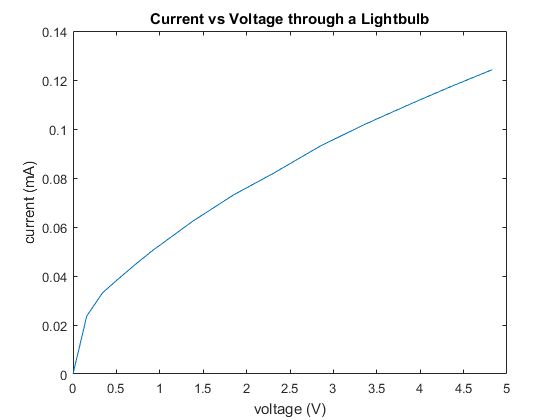
\includegraphics[scale = 0.8]{supplemental/lightbulbgraph.png}
			\caption{Finding the current vs voltage relationship in a light bulb through experimental tests with incremental increases in input voltage. As seen, the result was a nonlinear line.}
		\end{figure}

		\begin{figure}[H]
		\centering
		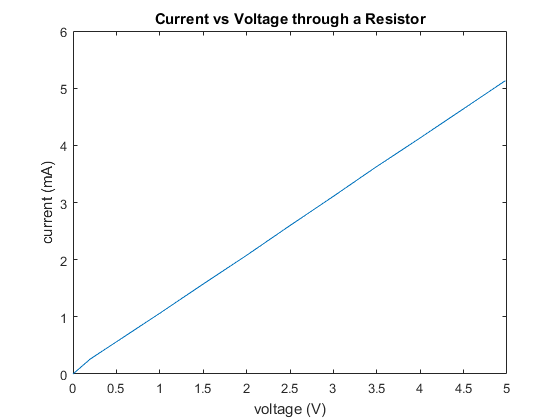
\includegraphics[scale = 0.8]{supplemental/resistorgraph.png}
		\caption{Finding the current vs voltage relationship in a 1 kOhm resistor through experimental tests with incremental increases in input voltage. As seen, the result was a linear line.}
		\end{figure}
		
		\begin{figure}[H]
			\centering
			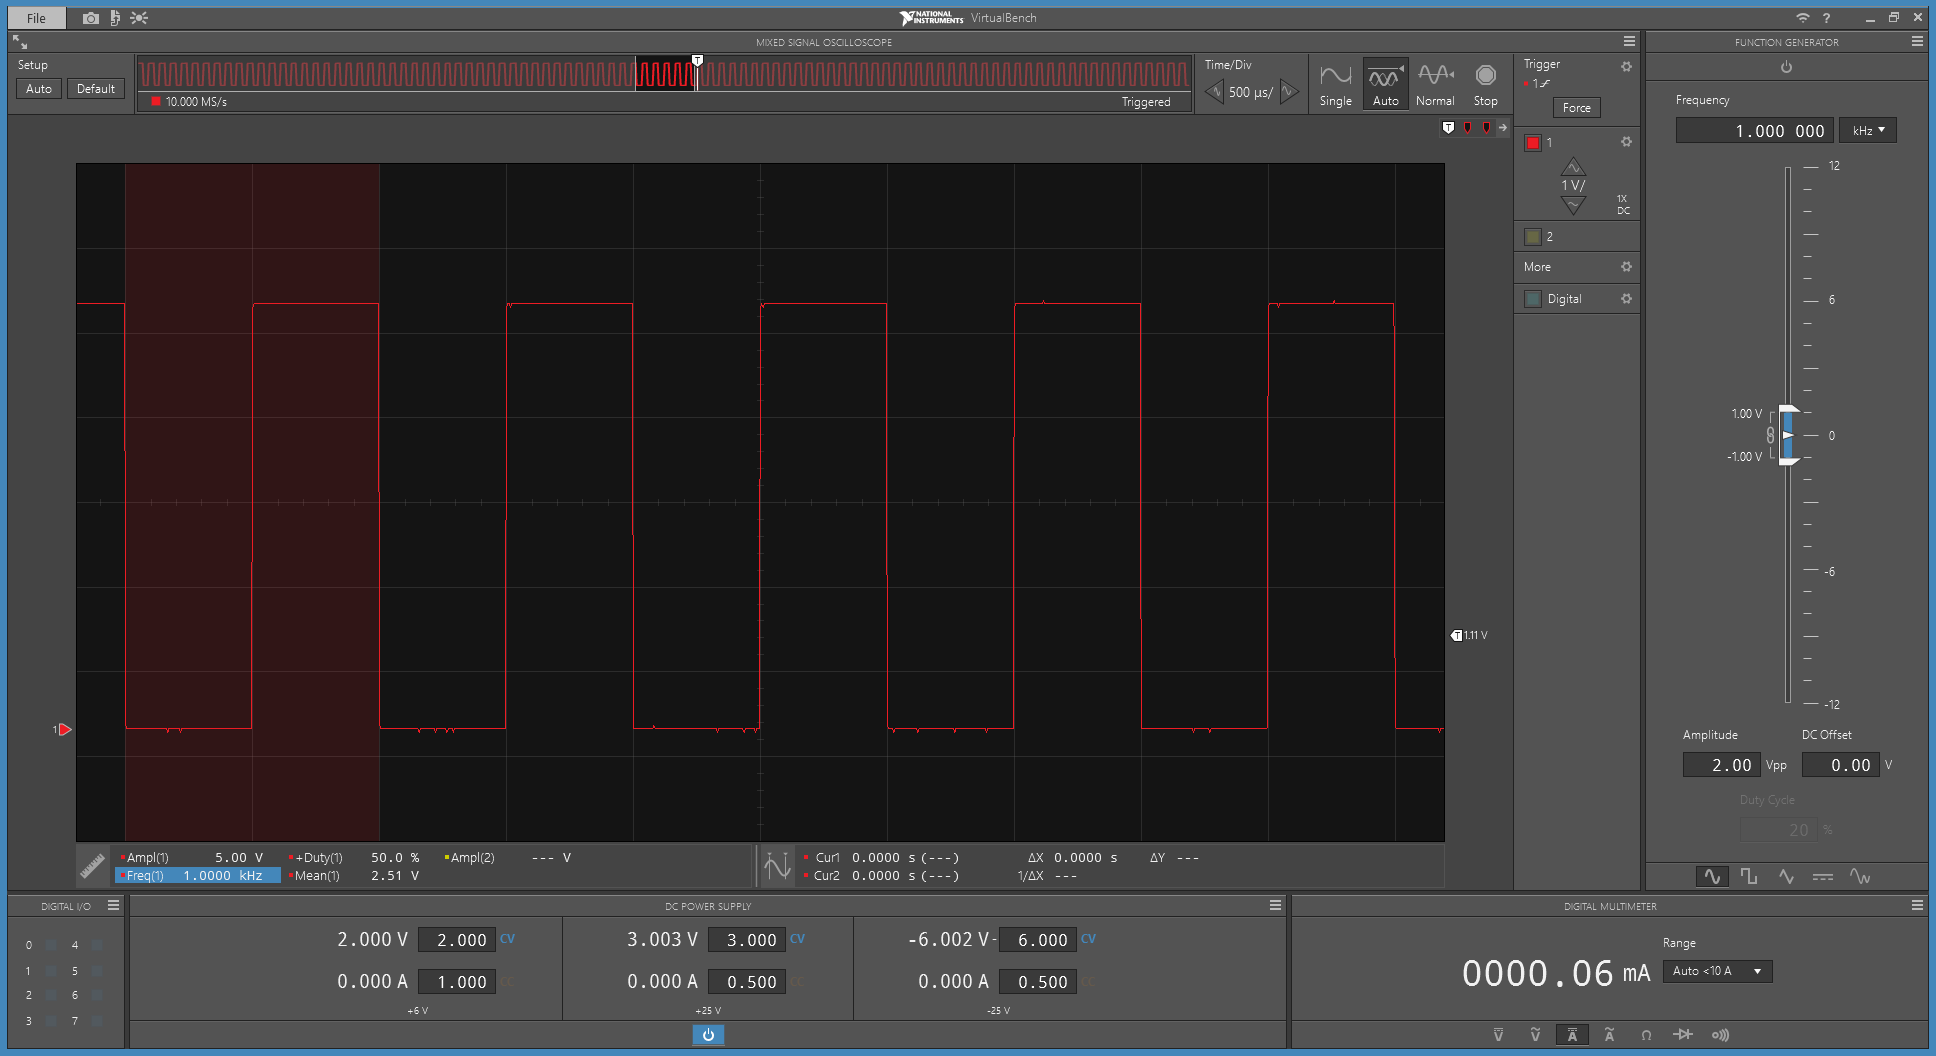
\includegraphics[scale = 0.35]{supplemental/squarewave.png}
			\caption{A print screen of the oscilloscope for a square wave created by the function generator, with a 50\% duty cycle. The shaded region represents a single period.}
		\end{figure}
	\end{center}


	
		
	\medskip
	
%	\textit{Note (To be deleted): Include the homework pre-calculations and schematics that serve as the initial setup for the test. Briefly explain the importance of each item you include. You may want to number your equations/figures so you can refer to them in later sections. Including photos of handwritten work is okay.}
	
	\section{Results and Discussion}
	
	\subsection{Experiment 1.1: The DMM}
	\subsubsection{Part A: Measuring Voltage with the DMM}

	Note: We were unable to aquire multiple Double A batteries for the initial tests
	\begin{itemize}
	
	\item Measuring the voltage of a D battery: 1.62V
	\item Voltage of battery attached to Lightbulb: 1.53V, The voltage has dropped, as some energy is being used to power the bulb
	\end{itemize}

	\subsubsection{Part B: Measuring Current with the DMM}
	\begin{itemize}
	\item Current across the battery in the Lightbulb - Battery circuit: 59.5 mA
	\item Current across the NC circuit: 59.1 mA
	\end{itemize}
	\subsubsection{Part C: Measuring Resistance with the DMM}
	\begin{itemize}
	\item 330 Ohms Resistor - Measured 325.7 Ohms
 430 Ohms Resistor - Measured 424 Ohms
 2200 Ohms Resistor - Measured 2153 Ohms
	\item All resistors had a tolerance of 5\%, which is in accordance with the measured values
	\item Holding the probes between your fingers opens a parallel path for the current to flow, which will lead to an inaccurate measure of the resistance of the circuit  
	\item The resistance of two resistors in series is 2R + 2d, where d is the tolerance of a single resistor
	\item The resistance of two resistors in parallel is .5R + .5d, where d is the tolerance of a single resistor
	\item Measuring 10 resistors with a resistance of 4.6 kOhms and a tolerance of 5\%
In kOhms: 4.61, 4.61, 4.59, 4.61, 4.63, 4.61, 4.63, 4.60, 4.61, 4.62. All of these resistances fall within the tolerance
	\item Resistance of the body through dry fingers: 1.325 MOhms with a resolution of .1 MOhms
	\item Resistance of the body throuh wet fingers: 168 kOhms with a resolution of 10 kOhms
	\item This change in resistance can be attributed to the fact that adding water to fingers increases the surface area of the contact of the leads to the skin, which leads to a decrease in resistance. Following Ohms law, with dry skin, a voltage of 6.625 kV would produce 5 mA of current
	\subsubsection{Part D: Measuring the I-V Characteristics of the Light Bulb}
	\item The resistance of the lightbulb is 4.8 Ohms. This is not the answer that we would expect from Ohm's law because a lightbulb is a non-Ohmic circuit element.
	\item The DMM reads .01 fewer volts that the Virtualbench power supply, hinting a voltage drop somewhere in the small circuit.
	\item For a  1kOhm resistor, Ohms Law holds for all V
	\end{itemize}

	\subsection{Experiment 1.2 The Oscilloscope and Function Generator}
	\subsubsection{Viewing Signals with te Oscilloscope}
	\begin{itemize}
	\item The numbers are slightly off from the function generator because of two factors, the first being that the generator is not perfectly able to create the given sine waves, and the second being that the oscilloscope uses various measurements and approximations to create its given outputs which cannot be perfectly accurate.
	\item The duty cycle changes the ratio of time spent on the positive pulse vs the negative pulse
	\item The DC offset shifts the curve along the Y axis
	\item The "DC" voltage used is actually just a recitified AC signal, and an oscilloscope can be used to find the effectiveness of the recifier.
	\item The comparison of the found frequency to the given frequency yields no surprises, with them being very similar.With a division of 100 microseconds per div, there is a period of 10 divisions, which is 1 millisecond. The given period (being the inverse of the given frequency) is .999 milliseconds It is within .001 ms.

	\end{itemize}

	\medskip
	
	\textit{Note (To be deleted): The heart of your report is the presentation of your results and a discussion of those results. In your discussion, you should not only analyze your results, but also discuss the implications of those results.}
	
	\section{References}
	
	\begin{enumerate}
		\item https://www.ece.rice.edu/~dpr2/elec240/lab1/
	\end{enumerate}
	
	\medskip
	
%\textit{Note (To be deleted): List any datasheets, websites, lab procedure, etc. used during the lab.}
	
	
	\section{Conclusion}
	\subsection{Experiment 1.1: The DMM}
	\qquad For Part A, we discovered that the voltage of the battery decreases when attached to a load because the internal resistance of the battery causes a voltage drop across the terminal when current flows through the battery. We learned that batteries are an approximation to an ideal voltage source, which means that the voltage will not remain constant when we draw current from the battery. \newline
	
	For Part B, we found that measuring the current in a circuit will cause the overall current of the circuit to decrease because the ammeter itself has an internal resistance that increases the overall resistance of the circuit. \newline
	
	For Part C, we found that almost none of the resistors were were equal to their stated resistance, likely because it is difficult to manufacture precise resistance values into resistors. However, we did find that all of them were within the stated tolerance range (which was 5\%). We also hypothesized that holding the leads to the probes between our fingers lead to inaccurate measurements because our fingers act as a parallel path for current to flow, leading to a less accurate measurement. \\
	Measuring the batch of 10 resistors reveals that they are very precise in their manufacture; all are within 1\% of the stated resistance despite the fact that their stated tolerance was 5\%. It was also shown the tolerance of two equivalent resistors in series was the same percentage as if those two resistors were in parallel, which is equivalent to the percentage tolerance of a single resistor.\\
	We then found that the resistance of a human body with wet fingers has a resistance of an order of magnitude less than a human body with dry fingers. We believe that the change of resistance with wet fingers occurs because water increases both the surface area of contact as well as the penetration of the leads into the skin, leading to higher electrical current with wet fingers over dry fingers. 
	\newline
	
	For Part D, we found that a lightbulb is a non-ohmic circuit element, as seen by Fig. 1 with the nonlinear relationship. Specifically, the current does not increase proportionally to voltage at higher voltages. 
	However, a resistor is an Ohmic circuit element, as seen by the linear line in Fig 2.
	
	\subsection{1.2: The Oscilloscope and Function Generator}
	For Part A, we found that the measurements from the oscilloscope were slightly different from the settings on the function generator because it is difficult for the function generator to create a perfect sine wave and also because the oscilloscope likely takes measurements at discrete intervals which leads to inaccuracies. \newline
	
	For Part B, we hypothesized that we can measure the DC power supply with an oscilloscope to see how constant the current that the power supply produces is. The current is not perfectly constant because the power supply must rectify wall AC power into direct current. When we observe the square wave with the oscilloscope, we noticed that 
	
	
	\medskip
	
	%textit{Note (To be deleted): While the ``Results and Discussion'' section focused on the test results individually, the ``Conclusion'' discusses the results in the context of the entire experiment. Usually, the objectives given in the ``Introduction'' are reviewed to determine whether the experiment succeeded. If the objectives were not met, you should analyze why the results were not as predicted.}
	
	\section{Errors}
	
	
	
	\medskip
	
	%\textit{Note (To be deleted): Briefly list sources of error and discuss how to eliminate or deal with them}
	
\end{document}
